\documentclass[a4paper]{article}

\usepackage[a4paper, top=8mm, bottom=8mm, left=8mm, right=8mm]{geometry}

\usepackage{float}
\usepackage{polyglossia}
\setdefaultlanguage[babelshorthands=true]{russian}
\setotherlanguage{english}

\usepackage{fontspec}
\setmainfont{FreeSerif}
\newfontfamily{\russianfonttt}[Scale=0.7]{DejaVuSansMono}

\usepackage[tiny, compact]{titlesec}

\usepackage{titling}
\setlength{\droptitle}{-1cm}
\pretitle{\begin{center}\begin{bfseries}\Large}
		\posttitle{\par\end{bfseries}\end{center}}
\preauthor{\begin{center}\normalsize}
	\postauthor{\par\end{center}\vspace{-1.8cm}}

\usepackage{hyperref}
\usepackage{bookmark}
\usepackage{csquotes}
\usepackage{graphicx} 
\usepackage{enumitem} 
\title{Постановка экспериментов на Spla}

\author{Ашихина Людмила Александровна}

\date{}

\begin{document}
	
	\maketitle
	
	\begin{flushright}
		Группа: \emph{25.Б42-мм}
		
		Кафедра: \emph{системного программирования}
		
		Научный руководитель: \emph{Григорьев Семен Вячеславович}
		
		Номер семестра практики: \emph{2}
	\end{flushright} 
	
\section{Постановка задачи}

Spla~--- \cite{spla} библиотека обобщённой разреженной линейной алгебры, предоставляющая средства для выполнения вычислений на GPU с использованием OpenCL~\cite{OpenCl}~--- открытого стандарта для программирования разнородных вычислительных систем. Библиотека предоставляет операции над разреженными матрицами и векторами и поддерживает подход к обработке графов на основе линейной алгебры.
	
Работа выполнялась в рамках задачи сравнительного исследования производительности Spla и CPU-аналога LAGraph~\cite{LAGraph}  на стандартных алгоритмах анализа графов. Требовалось провести серию измерений для различных графов и алгоритмов, сравнить время выполнения на GPU и CPU и определить сценарии, в которых использование GPU показывает преимущество.
	
\textbf{Целью работы является} сравнительная оценка производительности библиотек Spla и LAGraph при выполнении алгоритмов анализа графов на графах различной структуры и выявление случаев, в которых использование GPU обеспечивает преимущество по времени выполнения по сравнению с CPU.
	
Для достижения цели были поставлены следующие задачи:
\begin{enumerate}
\item Выбрать набор тестовых графов и алгоритмов анализа графов;
\item Провести серию измерений времени выполнения алгоритмов на Spla и LAGraph;
\item Сравнить полученные результаты для различных типов графов и алгоритмов.
\end{enumerate}
	
Результаты работы необходимы для формирования доказательной базы производительности Spla. Для конечных пользователей это позволит оптимизировать вычислительные процессы, выбирая устройство для конкретных типов графов и алгоритмов. Материалы исследования будут интегрированы в официальную документацию репозитория Spla в качестве тестов производительности.
\section{Описание предлагаемого решения}
В работе использовались готовые реализации алгоритмов BFS, SSSP, PageRank и Triangle Counting, предоставляемые библиотеками Spla и LAGraph. Для проведения сравнительного анализа был использован репозиторий \texttt{graph-bench}, позволяющий запускать алгоритмы на различных графах.
	
В рамках эксперимента оценивалось время выполнения четырёх алгоритмов:
\begin{itemize}[noitemsep]
\item \textbf{BFS} (поиск в ширину)~--- обход графа по уровням;
\item \textbf{SSSP} (Single Source Shortest Paths)~--- поиск кратчайших путей из одного источника;
\item \textbf{PR} (PageRank)~--- итеративный алгоритм оценки важности вершин;
\item \textbf{TC} (Triangle Counting)~--- подсчёт треугольников, то есть поиск циклов размера 3.
\end{itemize}
	
В качестве тестовых данных были выбраны 10 графов из коллекции SuiteSparse Matrix Collection репозитория graph-bench~\cite{graph-bench}: \texttt{coAuthorsCiteseer} (227k вершин, 1.6М рёбер), \texttt{coPapersDBLP} (541k вершин, 30.5М рёбер), \texttt{cit-Patents} (3.8М вершин, 33М рёбер), \texttt{amazon-2008} (735k вершин, 7М рёбер), \texttt{indochina-2004} (7.4М вершин, 302М рёбер), \texttt{belgium\_osm} (1.4М вершин, 3.1М рёбер), \texttt{roadNet-CA} (2М вершин, 5.5М рёбер), \texttt{road\_central} (14.1М вершин, 33.9М рёбер), \texttt{rgg\_n\_2\_22\_s0} (4.2М вершин, 60.7М рёбер), \texttt{rgg\_n\_2\_23\_s0} (8.4М вершин, 127М рёбер). Выбор графов позволяет сравнить производительность алгоритмов на данных из различных предметных областей и с различной структурой.
	
Эксперименты проводились на тестовом стенде со следующими характеристиками: CPU: AMD Ryzen 7 8845HS; GPU: AMD Radeon 780M; ОЗУ: 32 ГБ LPDDR5X; ОС: Ubuntu 24.04.4 LTS; OpenCL: 2.1. Использовалась версия библиотеки LAGraph 1.2.1.
	
В качестве сравниваемых вариантов использовались библиотека Spla,
выполнявшая вычисления на GPU, и библиотека LAGraph, выполнявшая
соответствующие алгоритмы на CPU. Для обеих библиотек использовались
одинаковые входные графы и соответствующие алгоритмы. Измерялось
время выполнения алгоритма. Для каждой пары \enquote{алгоритм~--- граф} параметры запуска оставались неизменными между повторными измерениями.

\section{Эксперименты}
Для сравнения производительности Spla и LAGraph измерялось время выполнения четырёх алгоритмов на выбранных графах. Для каждой пары «алгоритм — граф» было выполнено 20 замеров; результаты представлены в виде средних значений времени выполнения, измеряемое в миллисекундах. На графике представлены средние значения времени выполнения по результатам 20 замеров. 

\subsection{Результаты экспериментов}
Для каждой пары «алгоритм — граф» было выполнено 20 измерений времени выполнения. По результатам измерений рассчитывались среднее значение и выборочное стандартное отклонение. Разброс результатов оценивался относительно среднего времени выполнения; полученные значения использовались для оценки вариативности измерений при сравнении библиотек.

На рис.~\ref{fig:perf_comparison} показано сравнение времени выполнения исследованных алгоритмов. 
	
\begin{figure}[H]
\centering
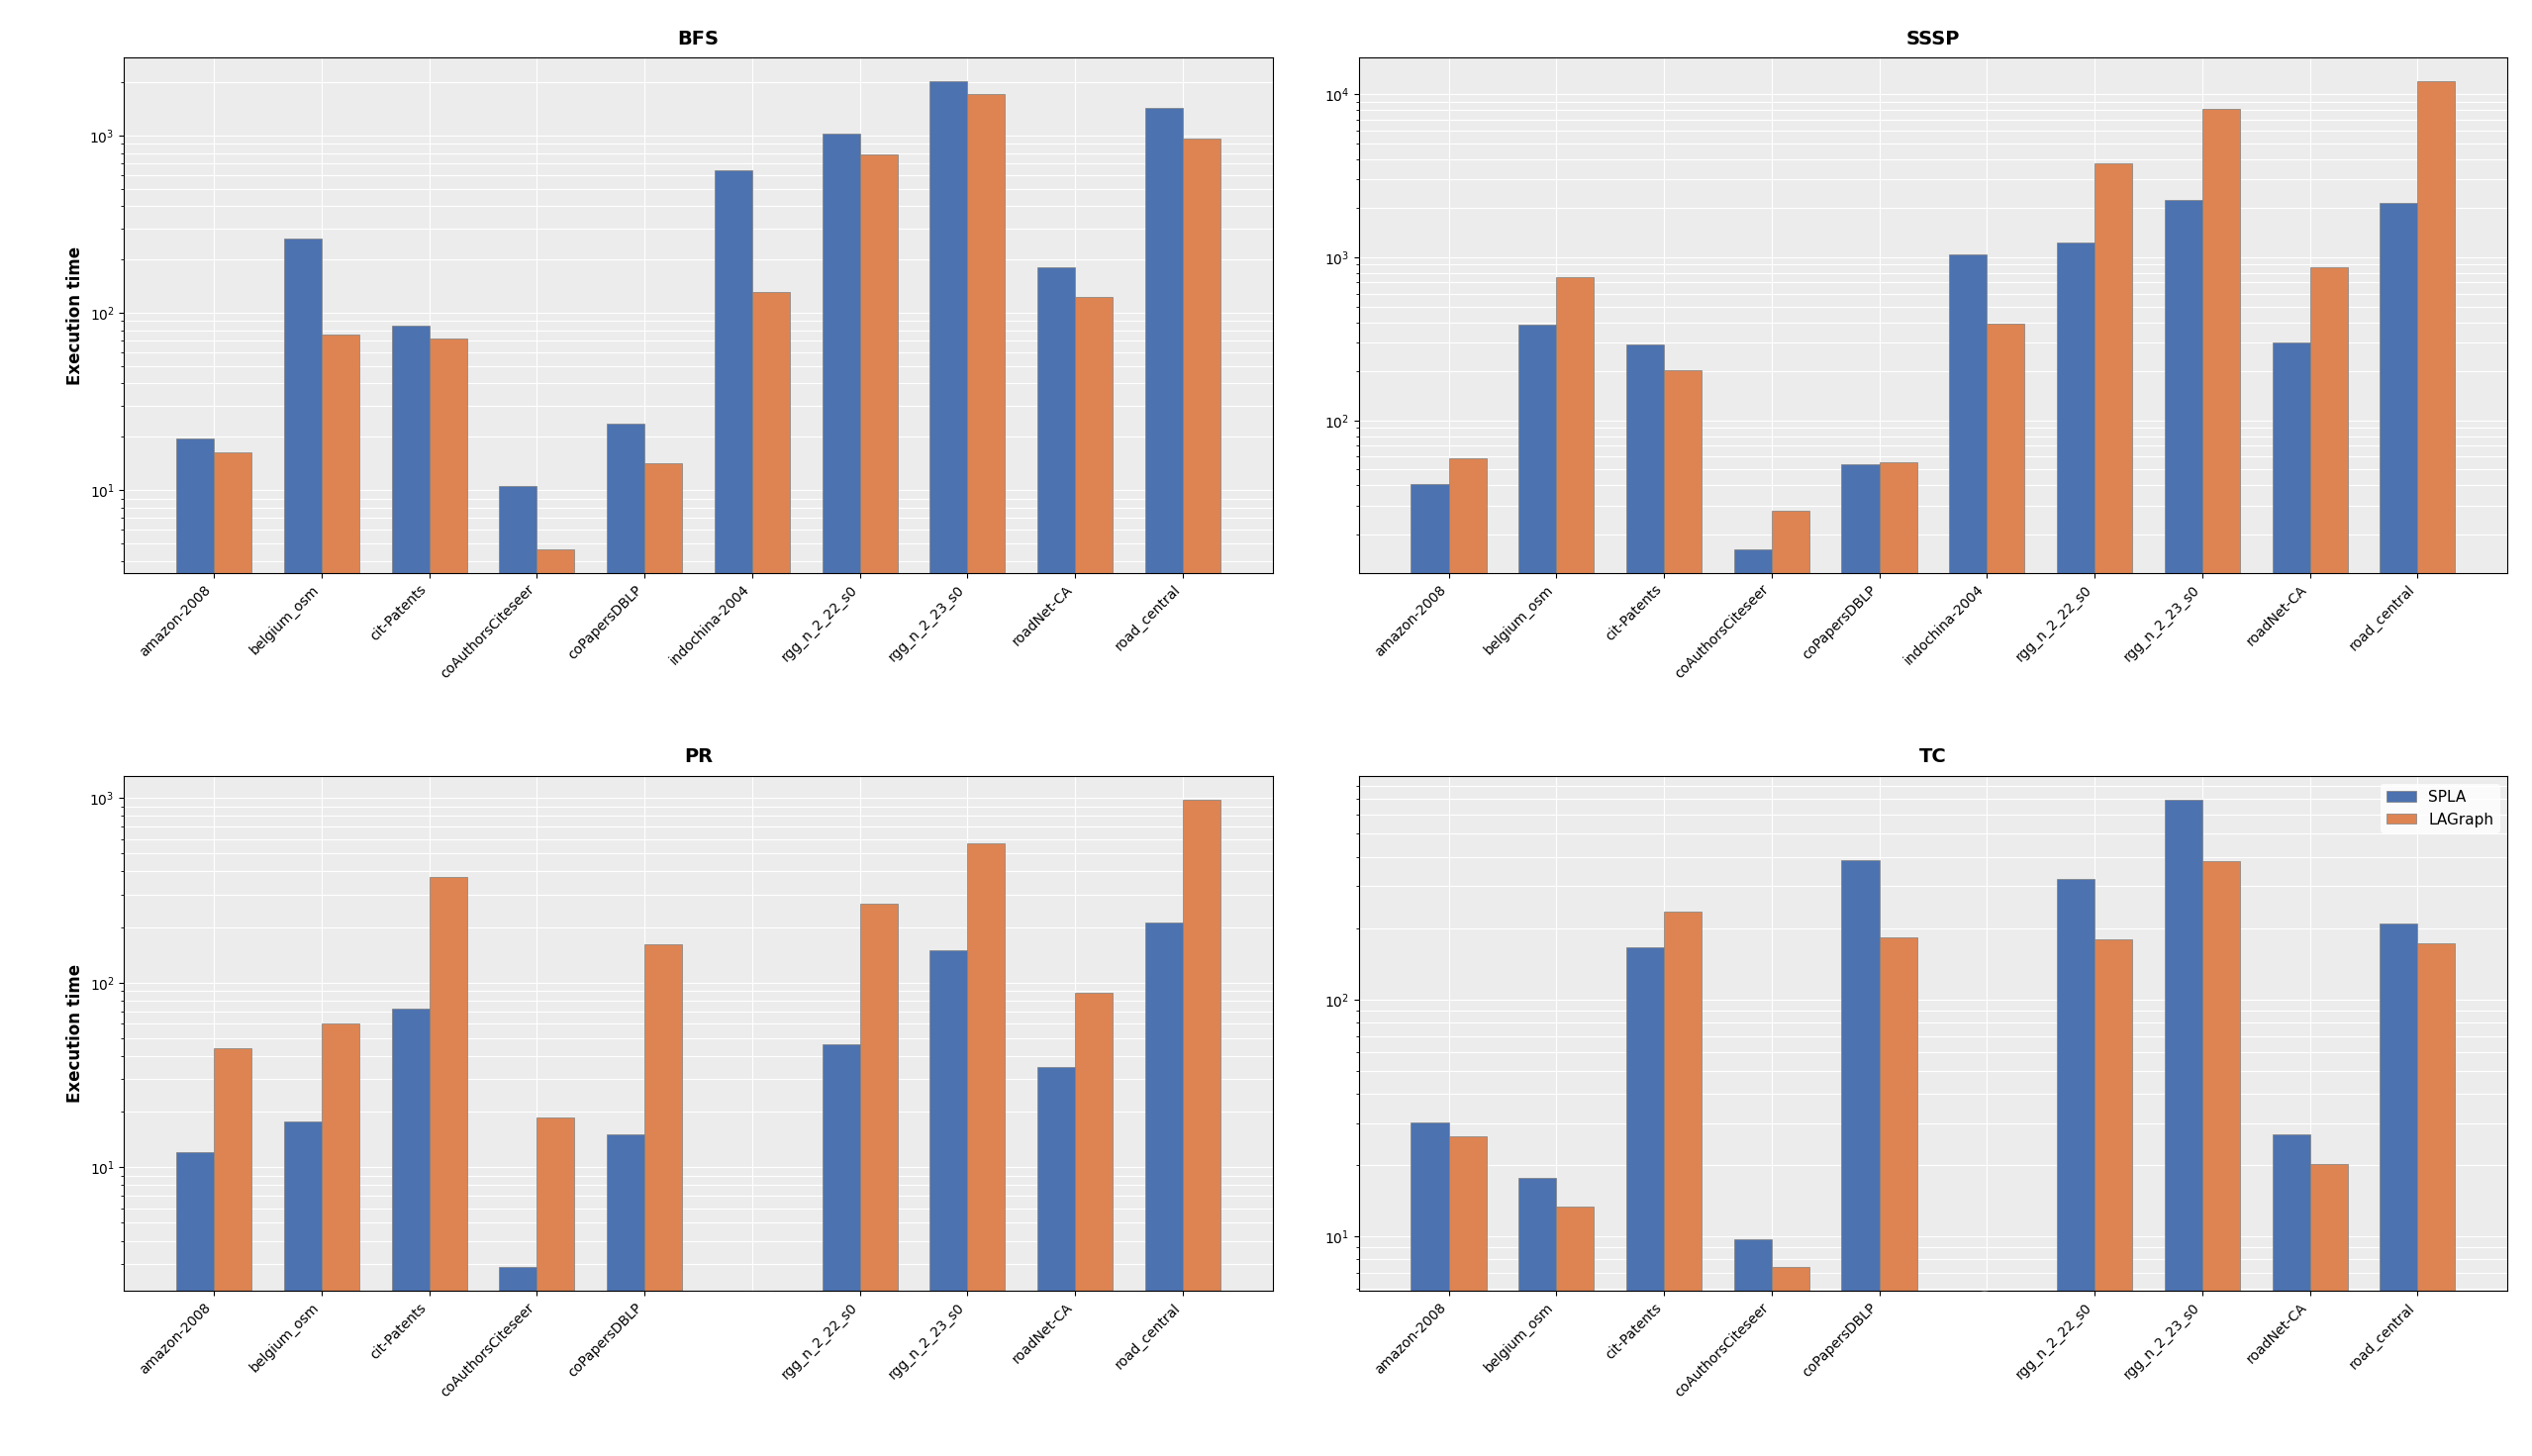
\includegraphics[width=1\textwidth]{graphic.png}
\caption{Сравнение времени выполнения алгоритмов}
\label{fig:perf_comparison}
\end{figure}
	
\subsection{Анализ результатов}
\begin{enumerate}
\item \textbf{PageRank (PR).}
Во всех исследованных случаях Spla показала меньшее время
выполнения по сравнению с LAGraph. Ускорение составило
от 2.53 до 10.70 раза. Наибольшая разница наблюдалась
на графе \texttt{coPapersDBLP}. Таким образом, на выбранном
наборе графов для PageRank было выявлено преимущество
исследованной GPU-реализации. Проведённые измерения
характеризуют различия во времени выполнения, но не
позволяют однозначно установить причины наблюдаемого
ускорения.
\item \textbf{SSSP (кратчайшие пути).}
Результаты зависят от входного графа. На графах
\texttt{road\_central}, \texttt{roadNet-CA},
\texttt{belgium\_osm}, \texttt{rgg\_n\_2\_22\_s0}
и \texttt{rgg\_n\_2\_23\_s0} меньшее время выполнения
показала Spla. На графах \texttt{cit-Patents} и
\texttt{indochina-2004} преимущество наблюдалось у
LAGraph. Следовательно, в рамках проведённого исследования
нельзя выделить одну реализацию как более быструю для
всех рассмотренных графов.
\item \textbf{Triangle Counting (TC).}
В большинстве исследованных случаев меньшее время
выполнения показала LAGraph. Исключением стал граф
\texttt{cit-Patents}, на котором более быстрое выполнение
продемонстрировала Spla. Этот результат показывает,
что соотношение производительности реализаций зависит
не только от выбранного алгоритма, но и от входных данных.
Для установления причин различий необходимы
дополнительные исследования.
\item \textbf{BFS (поиск в ширину).}
На всех десяти исследованных графах LAGraph показала
меньшее время выполнения, чем Spla. Наибольшая разница
наблюдалась на графе \texttt{indochina-2004}, где
CPU-реализация была быстрее примерно в 4.85 раза.
Таким образом, в рамках проведённых экспериментов
преимущество LAGraph для BFS наблюдалось независимо
от выбранного графа.
\end{enumerate}
Полученные результаты характеризуют соотношение времени выполнения исследованных реализаций, однако не позволяют установить причины наблюдаемых различий без дополнительных измерений.

\section{Заключение}
В ходе работы было проведено сравнение производительности библиотек Spla (GPU/OpenCL) и LAGraph (CPU) при выполнении четырёх алгоритмов анализа графов на десяти графах различной структуры. Для каждой пары «алгоритм — граф» было выполнено 20 измерений времени выполнения.

Результаты экспериментов показали, что преимущество одной библиотеки над другой зависит от используемого алгоритма. В исследованном наборе графов LAGraph продемонстрировала меньшее время выполнения BFS на всех графах, тогда как Spla показала меньшее время выполнения PageRank на всех графах, для которых были получены результаты. Для Triangle Counting преимущество LAGraph наблюдалось в большинстве исследованных случаев, а результаты SSSP зависели от входного графа.

Таким образом, в рамках проведённых экспериментов не выявлено универсального преимущества GPU-реализации над CPU-реализацией. Полученные результаты позволяют сравнить производительность исследованных реализаций на выбранном наборе графов и показывают, что выбор библиотеки следует рассматривать с учётом используемого алгоритма и входных данных.

Ссылка на репозиторий URL: \url{https://github.com/Lintari/Spla_experiments/tree/main}

Все результаты замеров и их средние значения доступны по ссылке: \url{https://github.com/Lintari/Spla_experiments/tree/main/analysis}

\begin{thebibliography}{99}
\bibitem{spla} Исходный код библиотеки Spla [Электронный ресурс] URL: https://github.com/SparseLinearAlgebra/spla (дата обращения: 20.09.2026).
\bibitem{OpenCl} Сайт проекта OpenCL [Электронный ресурс] URL: https://www.khronos.org/opencl/ (дата обращения: 20.09.2026).	
\bibitem{GraphBlas} GraphBLAS [Электронный ресурс] URL: https://github.com/GraphBLAS (дата обращения: 20.09.2026).
\bibitem{LAGraph} Исходный код библиотеки LAGraph [Электронный ресурс] URL: https://github.com/GraphBLAS/LAGraph (дата обращения: 20.09.2026).
\bibitem{graph-bench} Исходный код библиотеки graph-bench [Электронный ресурс] URL: https://github.com/EgorOrachyov/graph-bench (дата обращения: 20.09.2026).
\end{thebibliography}
\end{document}
